\chapter{Quantum Computing}
L'informatica quantistica combina l'informatica tradizionale con la meccanica quantistica ed è un campo di ricerca in rapida crescita. Questo interesse verso il calcolo quantistico inizia negli anni settanta con lo sviluppo di una serie di tecniche per ottenere il controllo completo di singoli sistemi quantistici. 

Fino a quel momento, la teoria classica dell'informatica era stata fondata sulla tesi ampiamente accettata di Church-Turing, secondo la quale era possibile teorizzare una macchina ideale, nota come \textit{Macchina di Turing}, capace di simulare in modo efficiente qualsiasi modello di calcolo esistente.

Tuttavia, l'emergente paradigma di calcolo basato sulle proprietà meccaniche quantistiche della natura portò molti scienziati a realizzare che, mentre un computer ordinario poteva essere usato per simulare un computer quantistico, era impossibile eseguire questa simulazione in modo efficiente: ogni tentativo di simulare l'evoluzione di un generico sistema fisico-quantistico su una macchina di Turing sembrava richiedere un overhead esponenziale di risorse.

R. P. Feynman fu tra i primi fisici ad occuparsi della questione, dando le linee guida sul possibile utilizzo di sistemi quantistici come costituenti di un nuovo tipo di calcolatore; sottolineò, inoltre, come un calcolatore di questo tipo sarebbe allo stesso tempo un "simulatore" ideale per i sistemi quantistici. A partire dalle osservazioni sviluppate in quel periodo, si iniziò a costruire una nuova teoria dell'informazione, che tenesse conto delle possibilità, ancora teoriche, offerte dal calcolatore quantistico. In particolare, una nuova classificazione della complessità computazionale si rese necessaria, grazie alle peculiarità ed ai vantaggi offerti dal nuovo paradigma computazionale.

Contributi fondamentali sono stati dati da David Deutsch che, nel 1985, si chiese se le leggi della fisica quantistica potessero essere usate per derivare una versione ancora più forte della tesi di Church-Turing e tentò di definire un dispositivo computazionale che fosse capace di simulare in modo efficiente un sistema fisico arbitrario. Questo dispositivo sarebbe diventato la moderna concezione di un computer quantistico e che questi dispositivi potssero avere poteri di calcolo ben superiori a quelli dei computer tradizionali, indipendentemente dai loro progressi ottenibili nel calcolo classico.

Negli anni seguenti, lo studio degli algoritmi quantistici si è evoluto come un sotto-campo dell'informatica quantistica con applicazioni di diverso tipo: ricerca e ottimizzazione, machine learning, simulazione di sistemi quantistici e crittografia.

Quest'ultimo campo è quello che più ci interessa, infatti, nel 1994 Peter Shor pubblica l'algoritmo che porta il suo nome per la fattorizzazione degli interi in tempo polinomiale.\cite{breaking-rsa} Questo è stato una svolta epocale nella materia, perché un importante metodo di crittografia asimmetrica noto come RSA si basa sulla supposizione che la fattorizzazione degli interi sia difficile dal punto di vista computazionale. L'esistenza dell'algoritmo quantistico in tempo polinomiale può dimostrare che uno dei protocolli crittografici più usati al mondo sarebbe vulnerabile a un computer quantistico.

\section{Il Quantum Bit}
\subsection{Definizione di quantum bit}
L'informazione non può essere considerata separatamente dalla sua natura fisica: non si può, cioè, mantenere, modificare o trasmettere informazione senza un adeguato supporto fisico. Nei computer tradizionali viene utilizzato come modello fondamentale il \textit{bit}, che rappresenta un sistema a due stati, 0 e 1. La scelta della rappresentazione binaria è dettata dalla semplicità e comodità di realizzazione nei sistemi elettronici. Il bit classico, quindi, mantiene correttamente l'informazione relativa ad una scelta esclusiva tra i due stati possibili in cui si può trovare (con \textit{n} bit possiamo rappresentare \(2^n\) stati).

La computazione quantistica introduce una nuova unità fondamentale che prende il nome di \textit{quantum bit}, chiamato anche \textit{qubit}. Un qubit usa i fenomeni meccanici quantistici della sovrapposizione per ottenere una combinazione lineare di due stati. Un bit binario classico può rappresentare solo un singolo valore binario, ad esempio 0 o 1, ovvero può trovarsi solo in uno di due stati possibili. Un qubit tuttavia può rappresentare uno 0, un 1 o qualsiasi proporzione di 0 e 1 nella sovrapposizione di entrambi gli stati, con una determinata probabilità che si tratti di uno 0 e una determinata probabilità che si tratti di un 1.

Fisicamente viene rappresentato con un sistema microscopico a due livelli come lo spin di una particella, la polarizzazione di un singolo fotone o due stati di un atomo ottenibili cambiando il livello energetico di un suo elettrone.

Se volessimo descriverlo matematicamente potremmo definirlo come un vettore unitario descritto in uno spazio vettoriale di Hilbert complesso bidimensionale (\(\mathbb{C}^2\)).

Per rappresentare gli elementi di uno spazio vettoriale complesso è conveniente utilizzare \textbf{la notazione di Dirac} (notazione standard della meccanica quantistica). Tale scelta è motivata dal fatto che quando si opera su un computer quantistico reale si utilizzano numerosi qubit, la cui rappresentazione sotto forma di vettore diventerebbe estremamente difficoltosa.

L'algebra di Dirac comprende due tipi di vettori: \textbf{bra} e il suo vettore duale \textbf{ket}.

Un ket rappresenta un vettore colonna e viene utilizzato solitamente per descrivere lo stato di un sistema:

\[
  | a \rangle = \begin{pmatrix} \alpha \\ \beta \end{pmatrix}
\]

Mentre un bra rappresenta la coniugata trasposta del vettore colonna ket:

\[
  \langle a | = \begin{pmatrix} \alpha & \beta \end{pmatrix}
\]

Il prodotto scalare tra i due vettori si indica con \(\langle \alpha | \beta \rangle\) in modo che il prodotto formi un \textbf{braket}.

Definendo due vettori:

\[
  \begin{pmatrix} 1 \\ 0 \end{pmatrix}
  \begin{pmatrix} 0 \\ 1 \end{pmatrix}
\]

e associandoli rispettivamente agli stati \( | 0 \rangle\) e \( | 1 \rangle\), essi formano una base \textit{ortonormale}, cioè una base \textit{ortogonale} di vettori aventi \textit{norma 1}, nota come \textbf{base computazionale standard}.

Possiamo inoltre dare una definizione degli stati attraverso la forma matriciale (vettori colonne), ottenendo la seguente rappresentazione:

\[
  | 0 \rangle = \begin{bmatrix} 1 \\ 0 \end{bmatrix}
  | 1 \rangle = \begin{bmatrix} 0 \\ 1 \end{bmatrix}
\]

I due vettori appena introdotti corrispondono esattamente agli stati classici 0 e 1. A questo punto è bene specificare la principale differenza con il bit classico: un qubit, oltre a potersi trovare in uno degli stati fondamentali, potrà trovarsi contemporaneamente anche in un'altra qualsiasi combinazione di entrambi gli stati base.

Se definiamo \( | \psi \rangle \) la seguente combinazione lineare:

\[
  | \psi \rangle = \alpha | 0 \rangle + \beta | 1 \rangle
\]

dove \(\alpha\) e \(\beta\) rappresentano numeri complessi tali che valga:

\[
  \lvert \alpha \rvert ^2 + \lvert \beta \rvert ^2 = 1
\]

allora \( | \psi \rangle \) è un possibile stato del qubit la cui notazione algebrica equivalente sarà:

\[
  | \psi \rangle
  = \alpha \begin{pmatrix} 1 \\ 0 \end{pmatrix}
  + \beta \begin{pmatrix} 0 \\ 1 \end{pmatrix}
  = \begin{pmatrix} \alpha \\ \beta \end{pmatrix}
\]

Il che equivale a dire che \( | \psi \rangle \) si trova in una sovrapposizione di stati. Quando abbiamo a che fare con un bit classico possiamo sempre stabilire con assoluta certezza in quale dei due stati esso si trovi, nel caso di un qubit non possiamo determinare con altrettanta precisione il suo stato quantistico, ossia i valori esatti di \(\alpha\) e \(\beta\).

La meccanica quantistica ci dice che soltanto attraverso l'effettiva misurazione del sistema otterremo un valore discreto del qubit, più precisamente si dice che lo stato collasserà nello stato \( | 0 \rangle \) con probabilità \( \lvert \alpha \rvert ^2 \) o in \( | 1 \rangle \) con probabilità \( \lvert \beta \rvert ^2 \). Proprio per questa ragione, i due valori \(\alpha\) e \(\beta\) prendono il nome di \textbf{ampiezze di probabilità} (amplitudes). Una prima semplice sovrapposizione è definita dallo stato:

\[
  \frac{1}{\sqrt{2}} | 0 \rangle
  + \frac{1}{\sqrt{2}} | 1 \rangle
  = \frac{1}{\sqrt{2}} (| 0 \rangle + | 1 \rangle)
\]

il quale ci tornerà utile in seguito.

Dunque per ora possiamo immaginare che fino al momento della sua effettiva misurazione, un qubit avrà una probabilità del 50\% di trovarsi nello stato \( | 0 \rangle \) e un altro 50\% di trovarsi in \( | 1 \rangle \); come se lanciando una moneta essa continuasse a girare su sé stessa fino al momento in cui la guardiamo e ne osserviamo il valore.

\subsection{Rappresentazione geometrica di un qubit}
Per ottenere una visualizzazione geometrica utile per comprendere meglio i diversi stati in cui un qubit può trovarsi, utilizziamo una sfera di raggio unitario la cosiddetta \textbf{Sfera di Bloch}, introdotta dal fisico Felix Bloch.
Gli stati del qubit verranno collocati in punti precisi della superficie della sfera, associando quindi ad ogni stato un punto. Lo stato \( | 1 \rangle \) verrà collocato nel polo sud, lo stato \( | 0 \rangle \) nel polo nord. I punti che giacciono sull'equatore avranno una probabilità del 50\% di essere nello stato \( | 0 \rangle \) e 50\% di essere nello stato \( | 1 \rangle \) così le altre locazioni indicheranno gli altri stati di sovrapposizioni quantistiche di \( | 0 \rangle \) e \( | 1 \rangle \).

\begin{figure}[h]
  \centering
  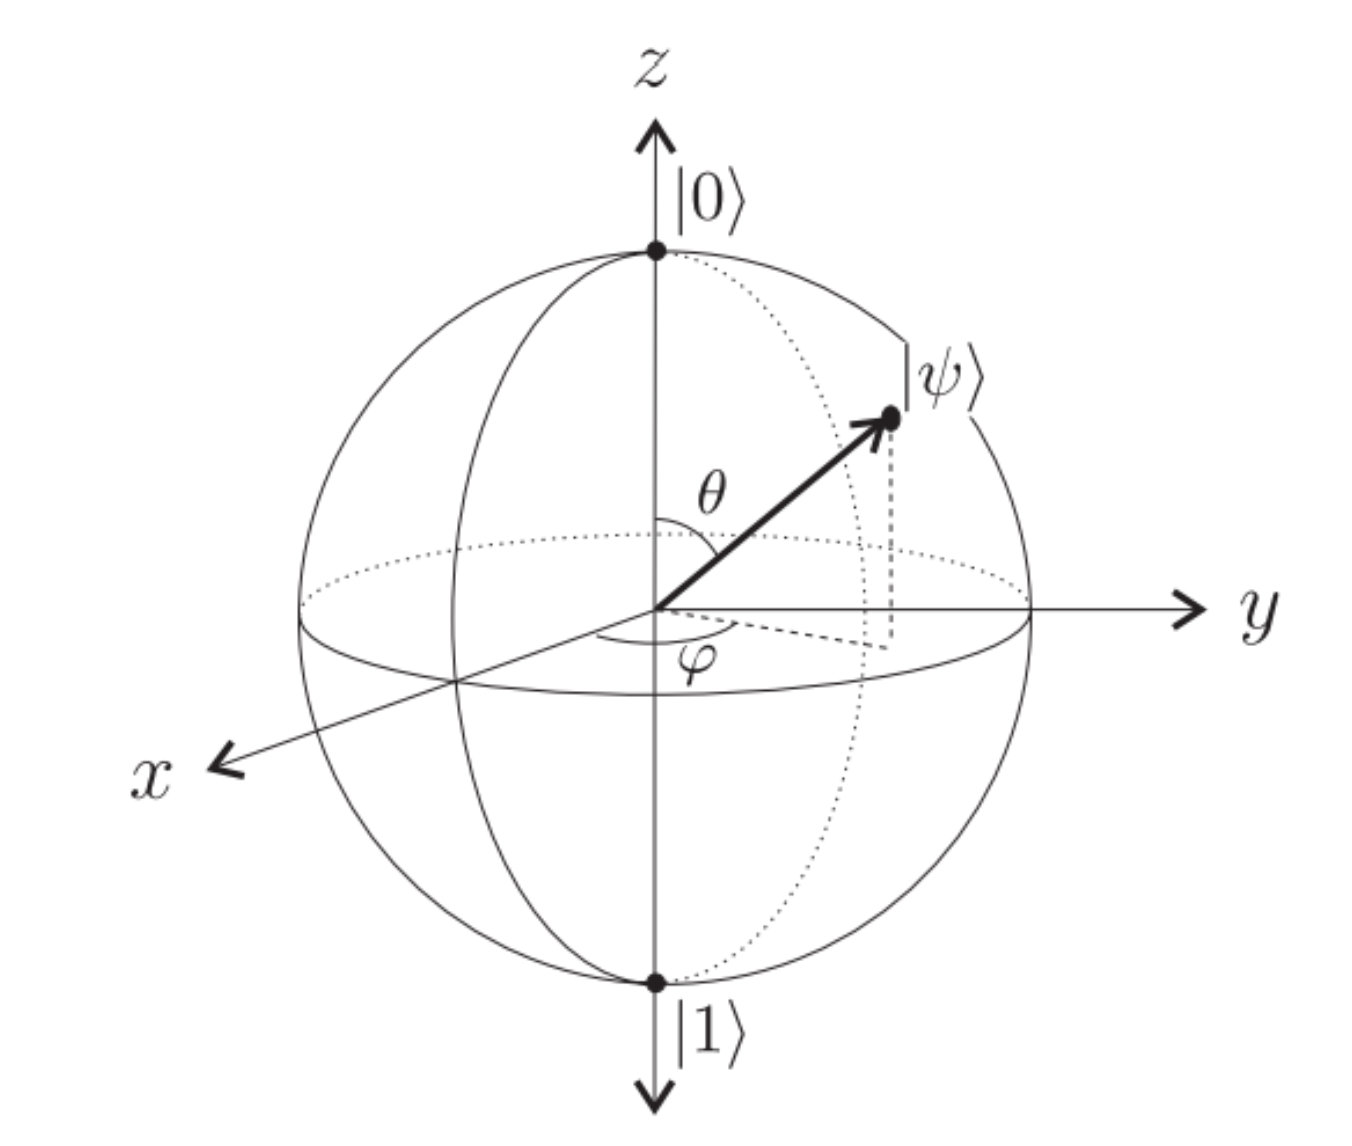
\includegraphics[width=0.7\textwidth]{qubit_geom.png}
  \caption{Rappresentazione di una Sfera di Bloch}
  \label{fig:qubit_geom}
\end{figure}

Come possiamo vedere nella figura \ref{fig:qubit_geom}, possiamo stabilire una corrispondenza biunivoca fra la rappresentazione generica dello stato di un qubit:

\[
  | \psi \rangle
  = \alpha | 0 \rangle
  + \beta | 1 \rangle
\]

E la sua rappresentazione sulla sfera unitaria in \( \mathbb{R} ^3 \):

\[
  | \psi \rangle
  = \cos \left( \frac{\theta}{2} \right)
  | 0 \rangle
  + e^{i\phi}
  \sin \left( \frac{\theta}{2} \right)
  | 1 \rangle
\]

Dove \( \theta \) e \( \phi \) sono le coordinate sferiche del punto. Si può quindi scrivere

\[
  | \psi \rangle
  = \alpha | 0 \rangle
  + e^{i\phi} \beta | 1 \rangle
\]

Dato che il vettore di stato ha norma 1

\[
  \sqrt{
    |\alpha|^2
    + |\beta|^2
  }
  = 1
\]

Si usa l'identità trigonometrica:

\[
  \sqrt{
    \sin^2 x
    + \cos^2 x
  }
  = 1
\]

Per descrivere \( \alpha \) e \( \beta \) reali in termini della variabile \( \theta \):

\[
  \alpha = \cos \left( \frac{\theta}{2} \right), 
  \beta = \sin \left( \frac{\theta}{2} \right)
\]

Da questo lo stato di ogni qubit si può descrivere usando le due variabili \(\theta\) e \(\phi\):

\[
  | \psi \rangle
  = \cos \left( \frac{\theta}{2} \right) | 0 \rangle
  + e^{i\phi} \sin \left( \frac{\theta}{2} \right) | 1 \rangle
\]

Interpretanto \(\theta\) e \(\phi\) come coordinate sferiche, si può tracciare qualsiasi stato del qubit sulla superficie della sfera di Bloch. In figura \ref{fig:qubit_stato} vengono visualizzati i seguenti vettori di stato del qubit:

\begin{figure}[h]
  \centering
  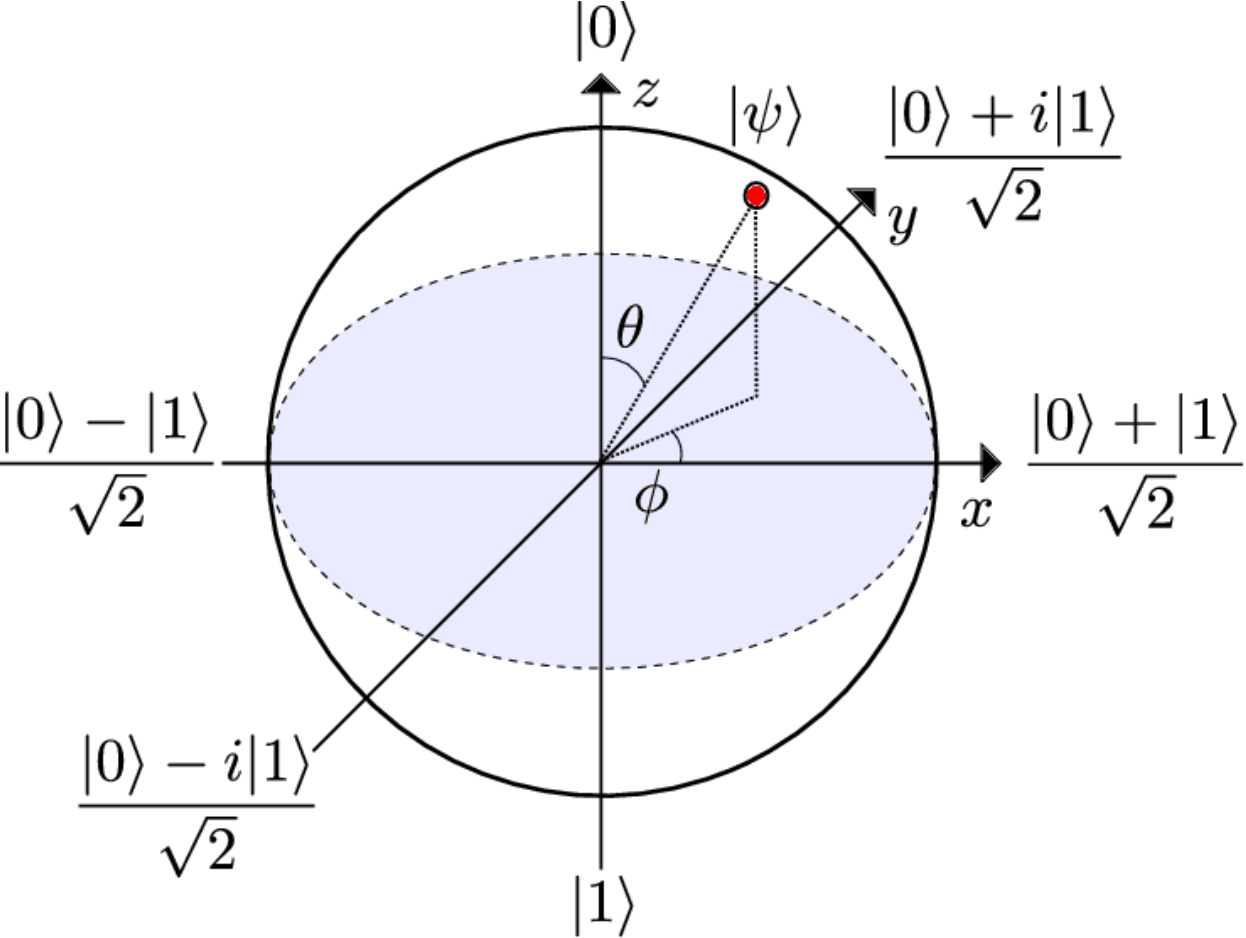
\includegraphics[width=0.7\textwidth]{qubit_stato.png}
  \caption{Visualizzazione dei qubit}
  \label{fig:qubit_stato}
\end{figure}

\begin{itemize}
  \item \( \begin{bmatrix} 1 \\ 0 \end{bmatrix} \) con \( \theta = 0 \) e \(\phi = 0\) cioè lo stato \( | 0 \rangle \)
  \item \( \begin{bmatrix} 0 \\ 1 \end{bmatrix} \) con \( \theta = 180 \) e \(\phi = 0\) cioè lo stato \( | 1 \rangle \)
  \item \( \begin{bmatrix} \frac{1}{\sqrt{2}} \\ \frac{i}{\sqrt{2}} \end{bmatrix} \) con \( \theta = \frac{\pi}{2} \) e \( \phi = \frac{\pi}{2} \)
  \item \( \begin{bmatrix} \frac{1}{\sqrt{2}} \\ \frac{1}{\sqrt{2}} \end{bmatrix} \) con \( \theta = \frac{\pi}{2} \) e \( \phi = 0 \) chiamato anche stato \( | + \rangle \)
  \item \( \begin{bmatrix} \frac{1}{\sqrt{2}} \\ \frac{-i}{\sqrt{2}} \end{bmatrix} \) con \( \theta = \frac{\pi}{2} \) e \( \phi = \frac{3\pi}{2} \)
  \item \( \begin{bmatrix} \frac{1}{\sqrt{2}} \\ \frac{-1}{\sqrt{2}} \end{bmatrix} \) con \( \theta = \frac{3\pi}{2} \) e \( \phi = 0 \) chiamato anche stato \( | - \rangle \)
\end{itemize}

Dato che in input inizialmente i qubit hanno sempre stato \( | 0 \rangle \), per poter operare sui qubit e ottenere degli stati differenti bisogna ruotare gli assi cardinali con le apposite \textit{porte logiche quantistiche}.

\section{Porte logiche quantistiche}
Esattamente come nel modello di computazione classica utilizziamo delle porte logiche come l'AND, OR o il NOT per effettuare delle operazioni tra bit, nel modello quantistico avremo delle porte che si occuperanno di manipolare i qubit per ottenere un risultato. In particolare ogni gate quantistico deve rispettare due criteri fondamentali:

\begin{itemize}
  \item \textbf{Reversibilità}: Un qubit a cui è stato applicato un cambiamento dello stato tramite l'utilizzo di una porta deve poter ritornare nello stato iniziale tramite l'applicazione della stessa porta all'output della prima.
  \item \textbf{Conservazione del vincolo di normalizzazione}: In questo modello, le porte logiche sono rappresentate da matrici unitarie. Una matrice quadrata \( U \) viene definita \textbf{unitaria} se vale \( UU^* = I \), dove \( U^* \) è la matrice \textbf{trasposta} e \( I \) è la \textbf{matrice identità}.
\end{itemize}

Proprio come nel modello classico, abbiamo sia porte logiche che agiscono su un singolo qubit, che porte che agiscono su più qubit.

\subsection{Porte Logiche a singolo qubit}
Contrariamente a quanto accade per le porte classiche, in ambito quantistico le porte a singolo bit non si limitano al \textbf{NOT}. Infatti abbiamo in totale quattro porte: \textbf{porta X}, \textbf{porta Y}, \textbf{porta Z} e \textbf{porta di Hadamard}. 

Le porte X, Y e Z prendono il nome di \textit{Porte di Pauli} e corrispondono a delle rotazioni rispettivamente sull'asse x, y e z della sfera di Bloch.

\subsubsection{Porta X}
Analoga alla porta NOT classica, la porta X svolge la stessa operazione del NOT classico invertendo lo stato del qubit nel caso sia uno degli stati base. La differenza con la porta classica sta nel fatto che il NOT nel modello quantistico si dovrà occupare anche di gestire degli stati sovrapposti che sono caratterizzati dai coefficienti \( \alpha \) e \( \beta \) del qubit.
Immaginando di rappresentare in forma vettoriale il qubit, e definendo la matrice corrispondente al NOT quantistico come:

\[
  X = 
  \begin{bmatrix}
    0 & 1 \\
    1 & 0
  \end{bmatrix}
\]

è facilmente verificabile che applicando tale porta a un qubit nella forma \( \alpha | 0 \rangle + \beta | 1 \rangle \) otterremo, seguendo la notazione vettoriale:

\[
  X
  \begin{bmatrix}
    \alpha \\ \beta
  \end{bmatrix}
  =
  \begin{bmatrix}
    \beta \\ \alpha
  \end{bmatrix}
\]

\begin{figure}[h]
  \centering
  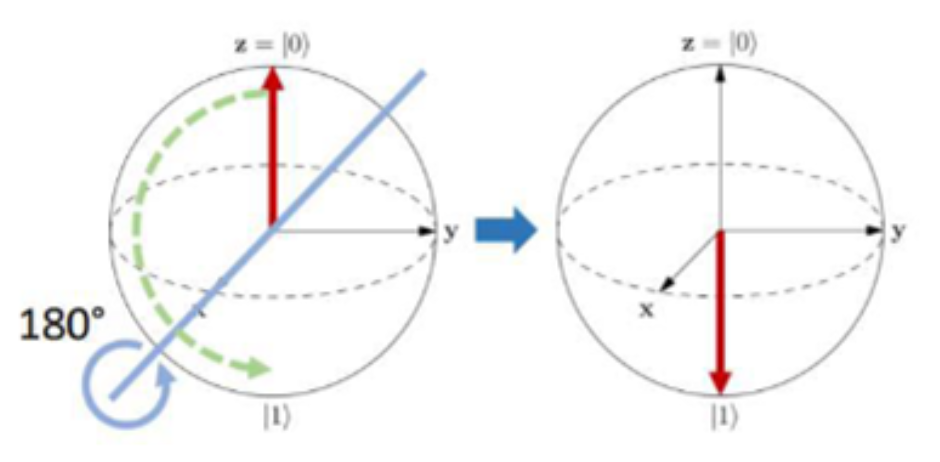
\includegraphics[width=0.7\textwidth]{gate_x.png}
  \caption{Visualizzazione dell'applicazione della Porta X}
  \label{fig:gate_x}
\end{figure}

\subsubsection{Porta Y}
La porta Y è rappresentata dalla seguente matrice:

\[
  Y
  =
  \begin{bmatrix}
    0 & -i \\
    -i & 0
  \end{bmatrix}
\]

che mappa la componente \( | 0 \rangle \) in \( i | 1 \rangle \) e la componente \( | 1 \rangle \) in \( -i | 0 \rangle \).

\begin{figure}[h]
  \centering
  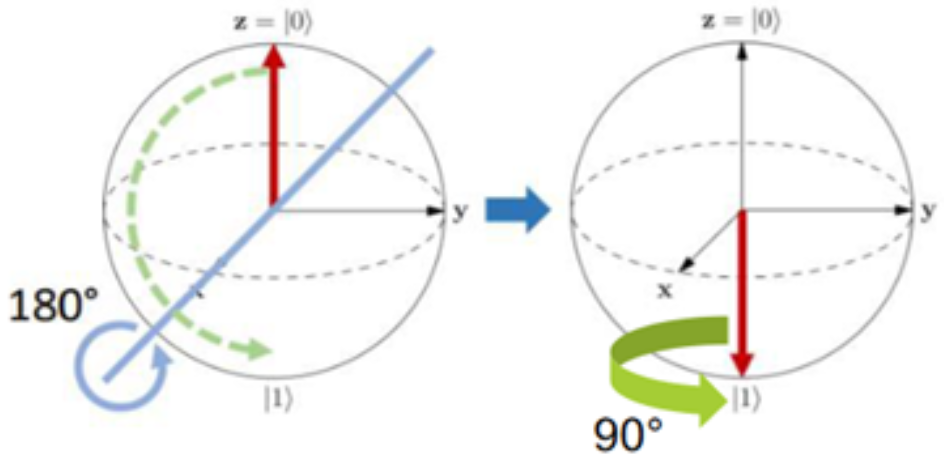
\includegraphics[width=0.7\textwidth]{gate_y.png}
  \caption{Visualizzazione dell'applicazione della Porta Y}
  \label{fig:gate_y}
\end{figure}

\subsubsection{Porta Z}
La porta Z è rappresentata dalla seguente matrice:

\[
  Z
  =
  \begin{bmatrix}
    1 & 0 \\
    0 & -1
  \end{bmatrix}
\]

che cambia il segno esclusivamente alla componente nello stato \( | 1 \rangle \).

\begin{figure}[h]
  \centering
  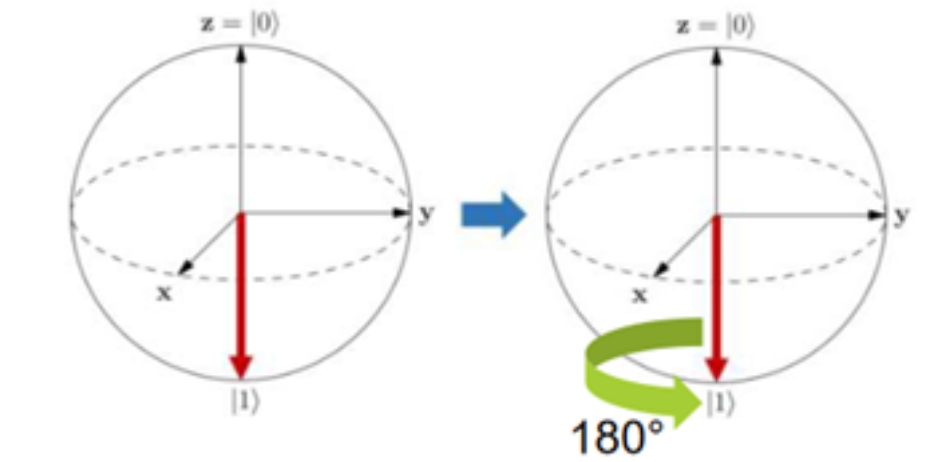
\includegraphics[width=0.7\textwidth]{gate_z.png}
  \caption{Visualizzazione dell'applicazione della Porta Z}
  \label{fig:gate_z}
\end{figure}

\subsubsection{Porta di Hadamard}
La porta di Hadamard è rappresentata dalla seguente matrice:

\[
  H
  =
  \frac{1}{\sqrt{2}}
  \begin{bmatrix}
    1 & 1 \\
    1 & -1
  \end{bmatrix}
\]

che si occupa di trasformare uno stato base in una sovrapposizione di tale stato che si trovi con il 50\% di probabilità in uno dei due stati fondamentali.

\begin{figure}[h]
  \centering
  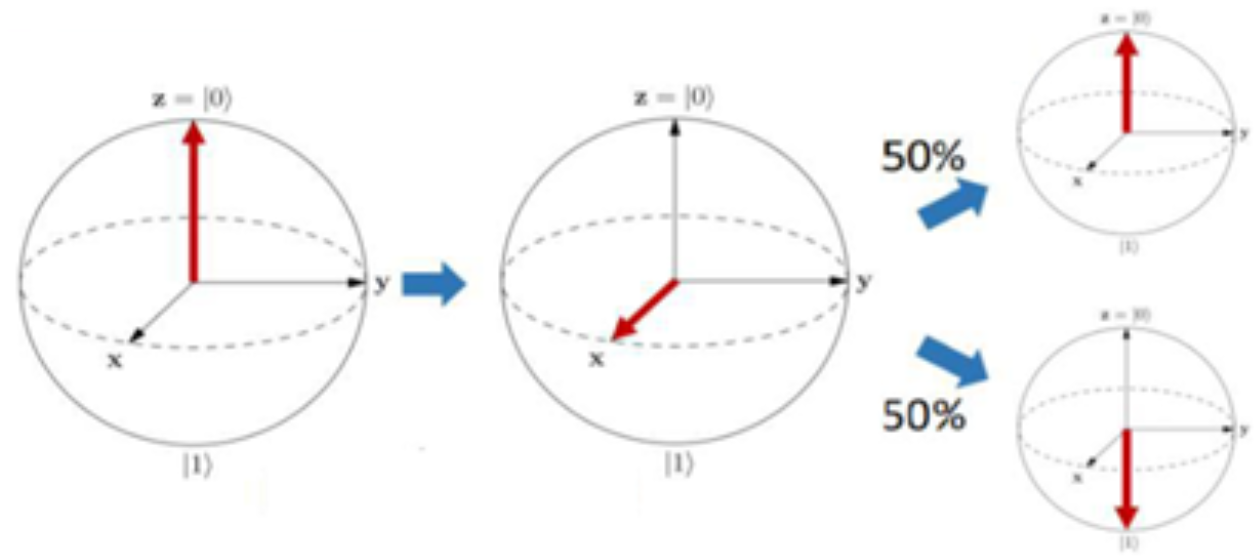
\includegraphics[width=0.7\textwidth]{gate_h.png}
  \caption{Visualizzazione dell'applicazione della Porta di Hadamard}
  \label{fig:gate_h}
\end{figure}

\subsection{Porte logiche a qubit multipli}
Proprio come nel modello di computazione classico, anche in questo modello siamo interessati ad avere un insieme di gate capaci di realizzare tutte le operazioni del modello classico. Nel caso del modello quantistico, per ottenere tale risultato, si affiancano le porte a singolo qubit con un operatore chiamato \textbf{CNOT} o \textbf{NOT Controllato}.

Il CNOT, che corrisponde allo XOR del modello classico, è dotato di due qubit in ingresso, rispettivamente definiti \textit{controllo} e \textit{bersaglio} (o \textit{target}). Dunque nel caso il qubit controllo si trovi nello stato zero allora il target viene lasciato inalterato, al contrario, se il qubit controllo è nello stato uno, allora il target viene invertito. Tale trasformazione può essere scritta come:

\[
  | A, B \rangle \mapsto | A, B \oplus A \rangle
\]

Il gate è rappresentato dalla seguente matrice:

\[
  CNOT = 
  \begin{bmatrix}
    1 & 0 & 0 & 0 \\
    0 & 1 & 0 & 0 \\
    0 & 0 & 0 & 1 \\
    0 & 0 & 1 & 0
  \end{bmatrix}
\]

Dove effettivamente possiamo notare come gli ultimi due stati vengano rispettivamente invertiti e prendendo in esempio un sistema composto da due qubit, il CNOT eseguirà operazioni mostrate in tabella \ref{tab:cnot}:

\begin{table}[htbp]
  \centering
  \begin{tabular}{|cc|cc|}
  \hline
  \multicolumn{2}{|c|}{Input} & \multicolumn{2}{c|}{Output} \\ \hline
  \multicolumn{1}{|c|}{Controllo} & Target & \multicolumn{1}{c|}{Controllo} & Target \\ \hline
  \multicolumn{1}{|c|}{\(|0\rangle\)} & \(|0\rangle\) & \multicolumn{1}{c|}{\(|0\rangle\)} & \(|0\rangle\) \\ \hline
  \multicolumn{1}{|c|}{\(|0\rangle\)} & \(|1\rangle\) & \multicolumn{1}{c|}{\(|0\rangle\)} & \(|1\rangle\) \\ \hline
  \multicolumn{1}{|c|}{\(|1\rangle\)} & \(|0\rangle\) & \multicolumn{1}{c|}{\(|1\rangle\)} & \(|1\rangle\) \\ \hline
  \multicolumn{1}{|c|}{\(|1\rangle\)} & \(|1\rangle\) & \multicolumn{1}{c|}{\(|1\rangle\)} & \(|0\rangle\) \\ \hline
  \end{tabular}
  \caption{Insieme delle possibili operazioni del gate CNOT}
  \label{tab:cnot}
\end{table}

Una delle proprietà fondamentali delle porte quantistiche, in particolare del CNOT e di tutte le porte viste a singolo qubit, è quella di essere invertibili, infatti a differenza delle porte classiche XOR e NAND generalmente irreversibili, permettono di ottenere l'input avendo a disposizione il valore di output. Combinando opportunamente CNOT e porte a singolo qubit, otteniamo l'insieme dei gate necessari per definire un insieme universale, capace dunque di inglobare le operazioni sufficienti alla rappresentazione di tutte le porte logiche quantistiche e quindi l'universalità delle operazioni quantistiche.

\section{Misurazione di un sistema di qubit}
Fin'ora abbiamo parlato di come vengono effettuate le operazioni sui qubit, tralasciando il modo in cui alla fine della computazione le informazioni sono raccolte. Immaginiamo che una particella sia dotata di un numero finito possibile di stati base e che tale particella li possegga tutti contemporaneamente fin quando non avviene l'evento della misurazione che farà ottenere uno degli stati base con probabilità uguale al quadrato del coefficiente associato a tale stato.

Nel nostro caso dato un qubit \(| \phi \rangle \) generico, il risultato di questa misurazione ci restituisce 0 con probabilità \( |\alpha|^2 \) e 1 con probabilità \( |\beta|^2 \).

Il problema in questo caso è che la misurazione disturba il qubit, lasciandolo nello stato \( | 0 \rangle \)  se il risultato della misurazione è 0, e nello stato \( | 1 \rangle \)  se il risultato della misurazione è 1.

In un circuito quantistico, a differenza della controparte classica, dopo la misurazione di un qubit esso viene scartato in quanto il suo stato essendo collassato, non è più valido.

Altra differenza con la controparte classica è il risultato della misurazione è la predicibilità ovvero che se l'esperimento effettuato venisse ripetuto rispettando le condizioni, ci aspetteremmo esattamente lo stesso risultato cosa che in ambito quantistico risulta incerta perché coadiuvata dal coefficiente associato allo stato.

\section{Registri quantistici}
Fin'ora abbiamo visto come rappresentare un solo qubit, per rappresentare un sistema a più qubit si utilizza un \textbf{registro quantistico}, che di fatto indica in che modo i qubit sono collegati tra loro. Per rappresentare questi registri si usa il \textbf{prodotto tensore} \( \otimes \), un operatore che combina spazi vettoriali di una certa dimensione per generarne dei più grandi, infatti: \( \otimes: \mathbb{C}^k \times \mathbb{C}^m \rightarrow \mathbb{C}^{km} \) quindi lo spazio totale di un registro quantistico sarà \( \mathbb{C}^{2 \cdot...\cdot 2} = \mathbb{C}^{2^n} \).

Formalmente si definisce un registro quantistico, secondo il quarto postulato della meccanica quantistica\footnote{Lo spazio degli stati di un sistema fisico composto è il prodotto tensore degli spazi degli stati dei sistemi fisici componenti. Se il sistema è composto da n sottosistemi e il componente i-esimo si trova nello stato \( | \phi _i \rangle \) allora lo stato del sistema totale è \( | \phi _1 \rangle \otimes | \phi _2 \rangle \otimes ... | \phi _n \rangle \)}, come:

\[
  | i _1 \rangle \otimes | i _2 \rangle \otimes ... | i _n \rangle
\]

dove \(i = 0,1\) e \(n\) è il numero di qubit e per convenienze possiamo rappresentare questo vettore semplicemente come \( | i _1 i _2 ... i _n \rangle \). Consideriamo un semplice sistema a due qubit, dove il primo è \( |\psi \rangle  = \alpha _0 |0 \rangle  + \beta _0 |1 \rangle \)  mentre il secondo \( |\theta \rangle  = \alpha _1 | 0 \rangle  + \beta _1 | 1 \rangle \) . Lo stato totale sarà una sovrapposizione dalla forma:

\[
  | \psi \rangle \otimes | \phi \rangle 
  = \alpha _{01} | 00 \rangle 
  + \alpha _0 \beta _1 | 01 \rangle 
  + \alpha _1 \beta _0 | 10 \rangle 
  +  \beta _{01} | 11 \rangle  
\]

Analogamente al singolo qubit dove il risultato della misurazione ci restituisce 0 con probabilità \( |\alpha|^2 \) e 1 con probabilità \( |\beta|^2 \). In un sistema di \(n\) qubit possiamo anche misurare solo un sottoinsieme degli \(n\) qubit. Ad esempio lo stato risulterà in \(| 00 \rangle \) con probabilità \( | \alpha _{01}|^2 \), in \(| 01 \rangle \) con probabilità \( | \alpha _0 \beta _1|^2 \) e così via. Inoltre se volessimo sapere la probabilità di ottenere 0 al primo bit basta sommare le probabilità di \(| 00 \rangle \) e \(| 01 \rangle \) cioè \( |\alpha _{01}|^2 + |\alpha _0 \beta _1|^2 \).

\section{Entanglement}
Dopo aver visto i registri quantistici una ulteriore proprietà legata ai possibili stati in cui può trovarsi il sistema è l'entanglement proprietà che non possiamo ritrovare in nessun oggetto della fisica classica. Questi stati chiamati entangled rappresentano quelle possibili configurazioni di n qubit componenti che non hanno un proprio stato ben definito ma solamente la loro combinazione ne rappresenta uno concreto. Più semplicemente uno stato entangled non può essere descritto come prodotto tensore degli stati dei singoli componenti.
Gli stati entangled si comportano come se fossero strettamente connessi l'uno all'altro indipendentemente dalla distanza fisica che li separa di modo che una misurazione o una operazione di uno dei due stati di una coppia entangled fornisce simultaneamente informazioni sulla coppia.
Un esempio per spiegare questa proprietà è dato dallo stato \( | 00 \rangle + | 11 \rangle \) che non può essere fattorizzato nel prodotto tensore di due qubit indipendenti, in quanto non esistono dei coefficienti \( \alpha _1 \alpha _2 \beta _1 \beta _2 \) tali per cui valga:
\[
  | 00 \rangle + | 11 \rangle
  = ( \alpha _1 | 0 \rangle + \beta _1 | 1 \rangle) \otimes ( \alpha _2 | 0 \rangle + \beta _2 | 1 \rangle)  
\]

\begin{figure}[h]
  \centering
  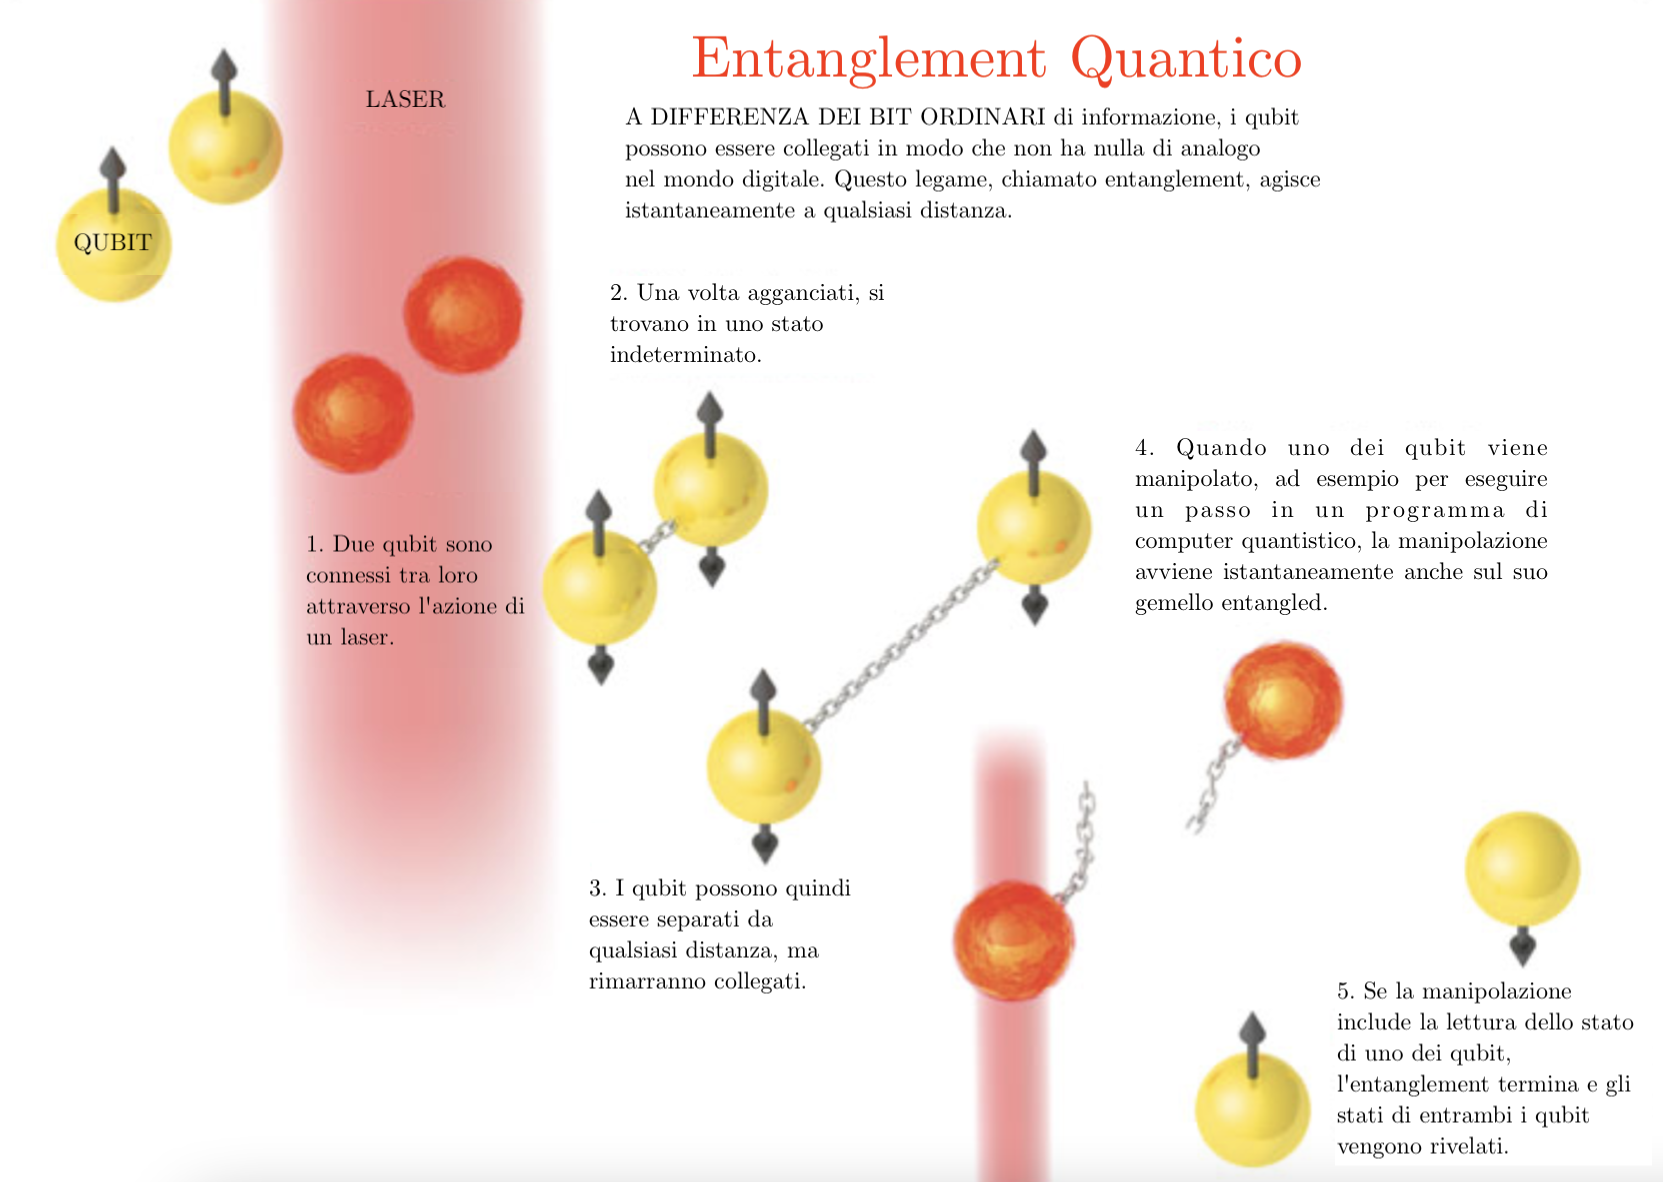
\includegraphics[width=0.7\textwidth]{entanglement.png}
  \caption{Visualizzazione degli effetti dell'entanglement}
  \label{fig:entanglement}
\end{figure}

L'entanglement è alla base della risoluzione di alcuni di quei problemi informatici non riproducibili classicamente grazie alla sua intrinseca proprietà non esistente nella fisica classica che da possibilità di ottenere un aumento esponenziale nella capacità di calcolo.

\section{Realizzazione di un computer quantistico}
Definiamo un computer quantistico come un calcolatore che segue il modello di computazione quantistico, sfruttando i dettami della fisica quantistica per eseguire dei calcoli che in alcuni casi risultano essere impossibili da realizzare in un calcolatore classico.

\subsection{Classi di complessità}
Prima di proseguire con l'introduzione delle componenti di un computer quantistico e bene tenere a mente le classi di complessità che non sono altro un insieme di problemi di una determinata complessità.
I problemi vengono eseguiti su una macchina di Turing per individuarne la particolare classe di complessità in cui rientrano. Le due classi più importanti sono \textbf{P} e \textbf{NP}.

\begin{figure}[h]
  \centering
  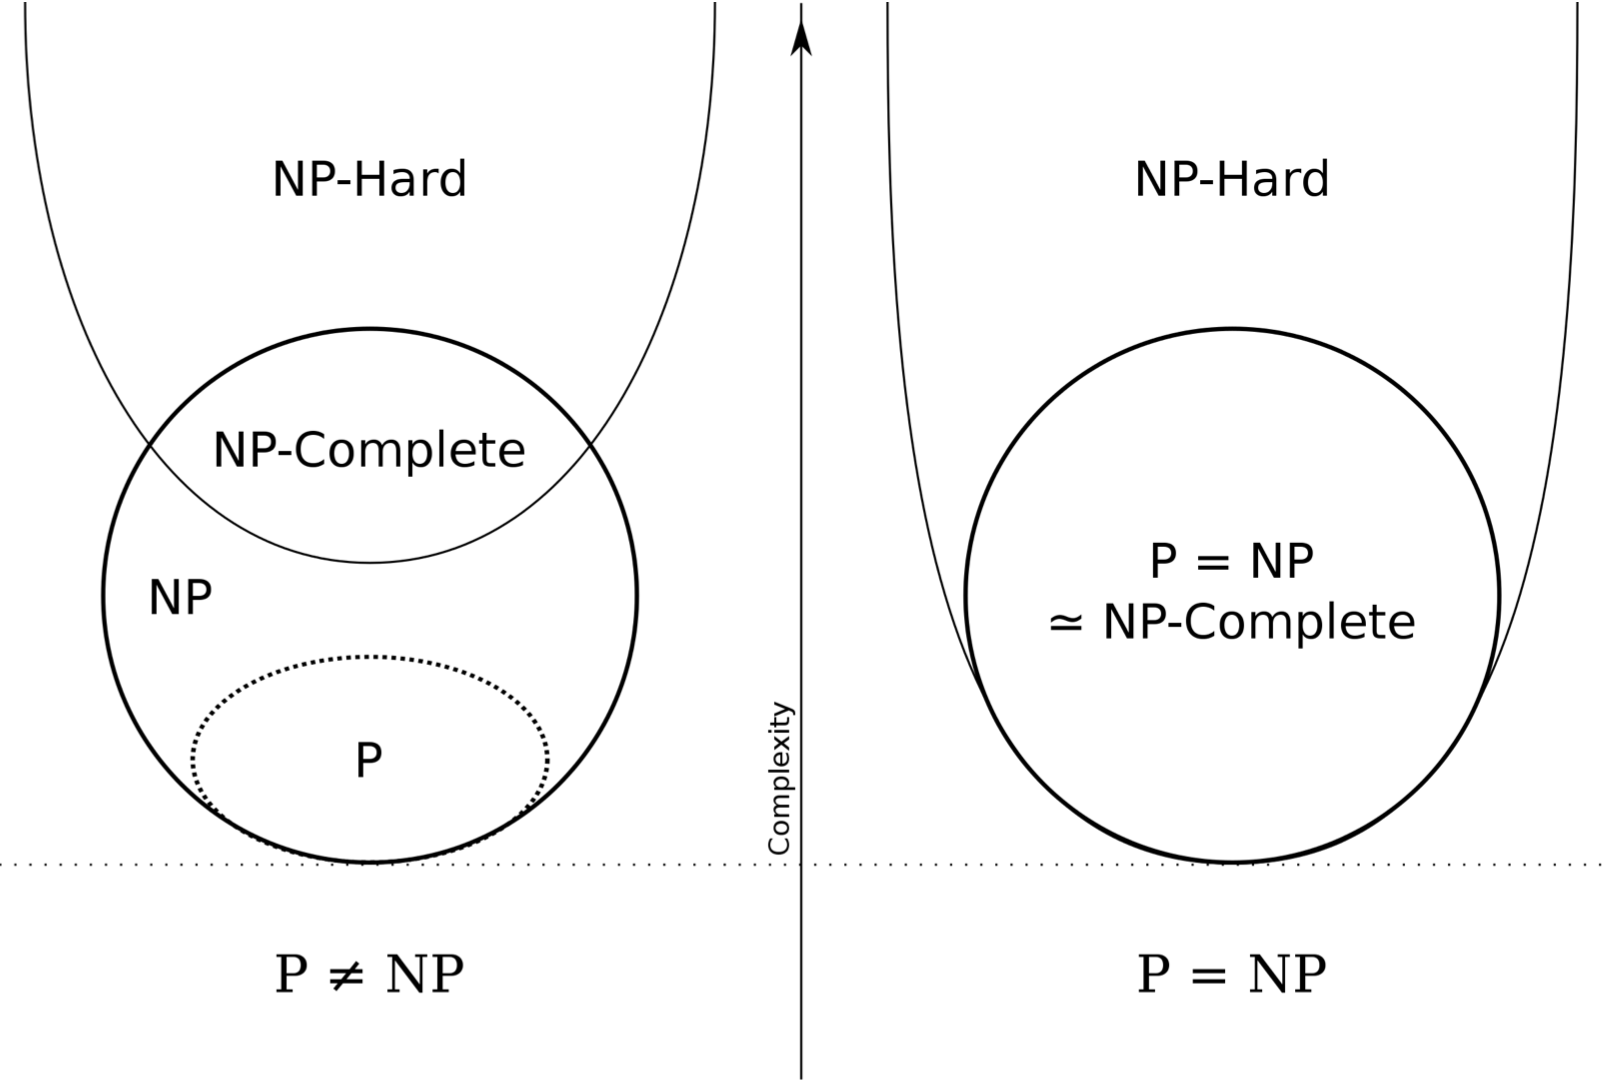
\includegraphics[width=0.7\textwidth]{complexity.png}
  \caption{Le classi di complessità per \(P = NP\) e \(P \neq NP\)}
  \label{fig:complexity}
\end{figure}

\begin{itemize}
  \item La classe \textbf{P} è l'insieme dei problemi di decisione che possono essere risolti da una macchina di Turing deterministica in tempo polinomiale.
  \item La classe \textbf{NP} è l'insieme dei problemi di decisione che possono essere risolti da una macchina di Turing non deterministica in tempo polinomiale. Inoltre nella classe NP è composta anche dalle classi NP-Complete e NP-Hard.
  \begin{itemize}
    \item La classe \textbf{NP-Complete} è l'insieme dei problemi più difficili nella classe NP nel senso che, se si trovasse un algoritmo in grado di risolvere "velocemente" (in tempo polinomiale) un qualsiasi problema NP-completo, allora si potrebbe usarlo per risolvere "velocemente" ogni problema in NP.
    \item In teoria della complessità, i problemi NP-difficili o NP-ardui sono una classe di problemi che può essere definita informalmente come la classe dei problemi almeno difficili come i più difficili problemi delle classi di complessità P e NP.
  \end{itemize}
\end{itemize}

Gli informatici \textit{Bernstein} e \textit{Vazirani} nel 1997 definirono una nuova classe di complessità chiamata \textbf{BQP} (\textit{Bounded-error Quantum Polynomial time}) che è la classe di complessità dei problemi decisionali che possono essere risolti con un errore bilaterale su una macchina di Turing quantistica in tempo polinomiale. In breve, tutti i problemi decisionali che i computer quantistici possono risolvere in maniera veloce. Inoltre, è stato dimostrato che \( P \in BPQ \) e quindi è semplice dedurre che i computer quantistici possono riolvere tutti i problemi che i computer classici possono risolvere.

\begin{figure}[htbp]
  \centering
  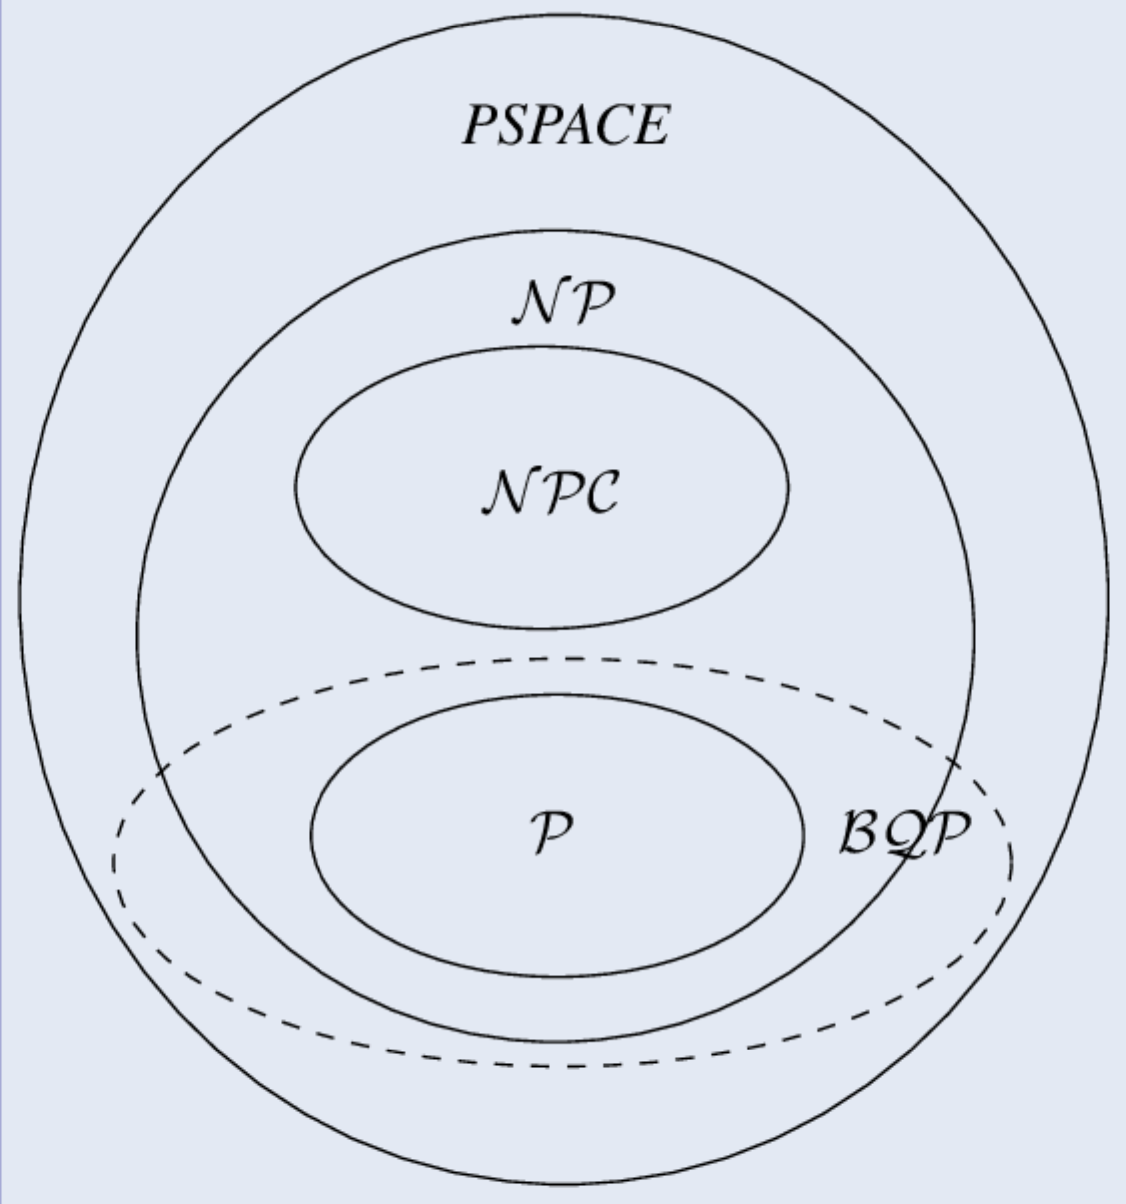
\includegraphics[width=0.7\textwidth]{bqp.png}
  \caption{La classe di complessità BQP rispetto a quelle classiche}
  \label{fig:bqp}
\end{figure}

\subsection{Macchina di Turing Quantistica}
La \textbf{Macchina di Turing Quantistica} (\textbf{QTM}) è stata descritta per la prima volta da Deutsch \cite{deutsch1985quantum}. L'idea di base è abbastanza semplice, un QTM è più o meno una Macchina di Turing probabilistica (PTM) con ampiezze di transizione complesse anzichè probabilità reali. A sua volta una Macchina di Turing Probabilistica (PTM) è identica a una normale Macchina di Turing tranne per il fatto che ad ogni configurazione della macchina (\(q_{i}S_{j}\)) c'è un insieme finito di regole di transizione (ognuna con una probabilità associata) che si applicano e che una scelta casuale determina quale regola applicare. Fissiamo una soglia di probabilità maggiore delle quote pari (diciamo, 75\%) e diciamo che una PTM specifica calcola \(f(x)\) sull'input \(x\) se e solo se si ferma con \(f(x)\) come output con probabilità maggiore del 75\%.

\subsection{Condizioni per la realizzazione}
Per la realizzazione di un computer quantistico nel 2000 sono stati stilati dal fisico teorico Di Vincenzo i \textbf{criteri di DiVincenzo} \cite{DiVincenzo_2000} che consistono in sette condizioni necessarie per costruire un computer seguentdo il modello quantistico, le prime cinque sono necessarie per il calcolo quantistico e sono:

\begin{enumerate}
  \item Il sistema deve essere \textit{scalabile}, con qubit ben caratterizzati;
  \item Deve essere possibile preparare uno \textit{stato iniziale generico}, ad esempio \(| 0000 \rangle \). Diversamente, sarà impossibile introdurre dati nel computer;
  \item I \textit{Tempi di de-coerenza} devono essere abbastanza lunghi, per poter realizzare un numero sufficiente di operazioni sfruttando la correlazione quantistica;
  \item Occorre \textit{un insieme universale di porte quantistiche}, ovverosia si deve poter costruire una varietà sufficiente di porte quantistiche per permettere qualsiasi operazione logica;
  \item Si deve disporre di un modo per misurare lo stato dei qubit, senza il quale sarebbe impossibile estrarre l'informazione processata dal computer;
\end{enumerate}

Le restanti due servono per la comunicazione quantistica e sono:

\begin{enumerate}
  \setcounter{enumi}{5}
  \item Deve esserci un sistema per \textit{convertire i qubit} immagazzinati in qubit messaggeri, ovvero deve esistere un sistema per trasmettere informazioni;
  \item La capacità di \textit{trasmettere fedelmente} qubit tra le varie locazioni specificate, per la medesima ragione del punto precedente.
\end{enumerate}

Negli ultimi anni si stanno sperimentando vari modi per la realizzazione dei computer quantistici come:
\begin{itemize}
  \item Superconduttori
  \item Ioni intrappolati di un atomo o di una molecola
  \item Risonanza magnetica nucleare
  \item Quantum annealing o ricottura quantistica
  \item Silicium quantum dot
\end{itemize}

\begin{figure}[htbp]
  \centering
  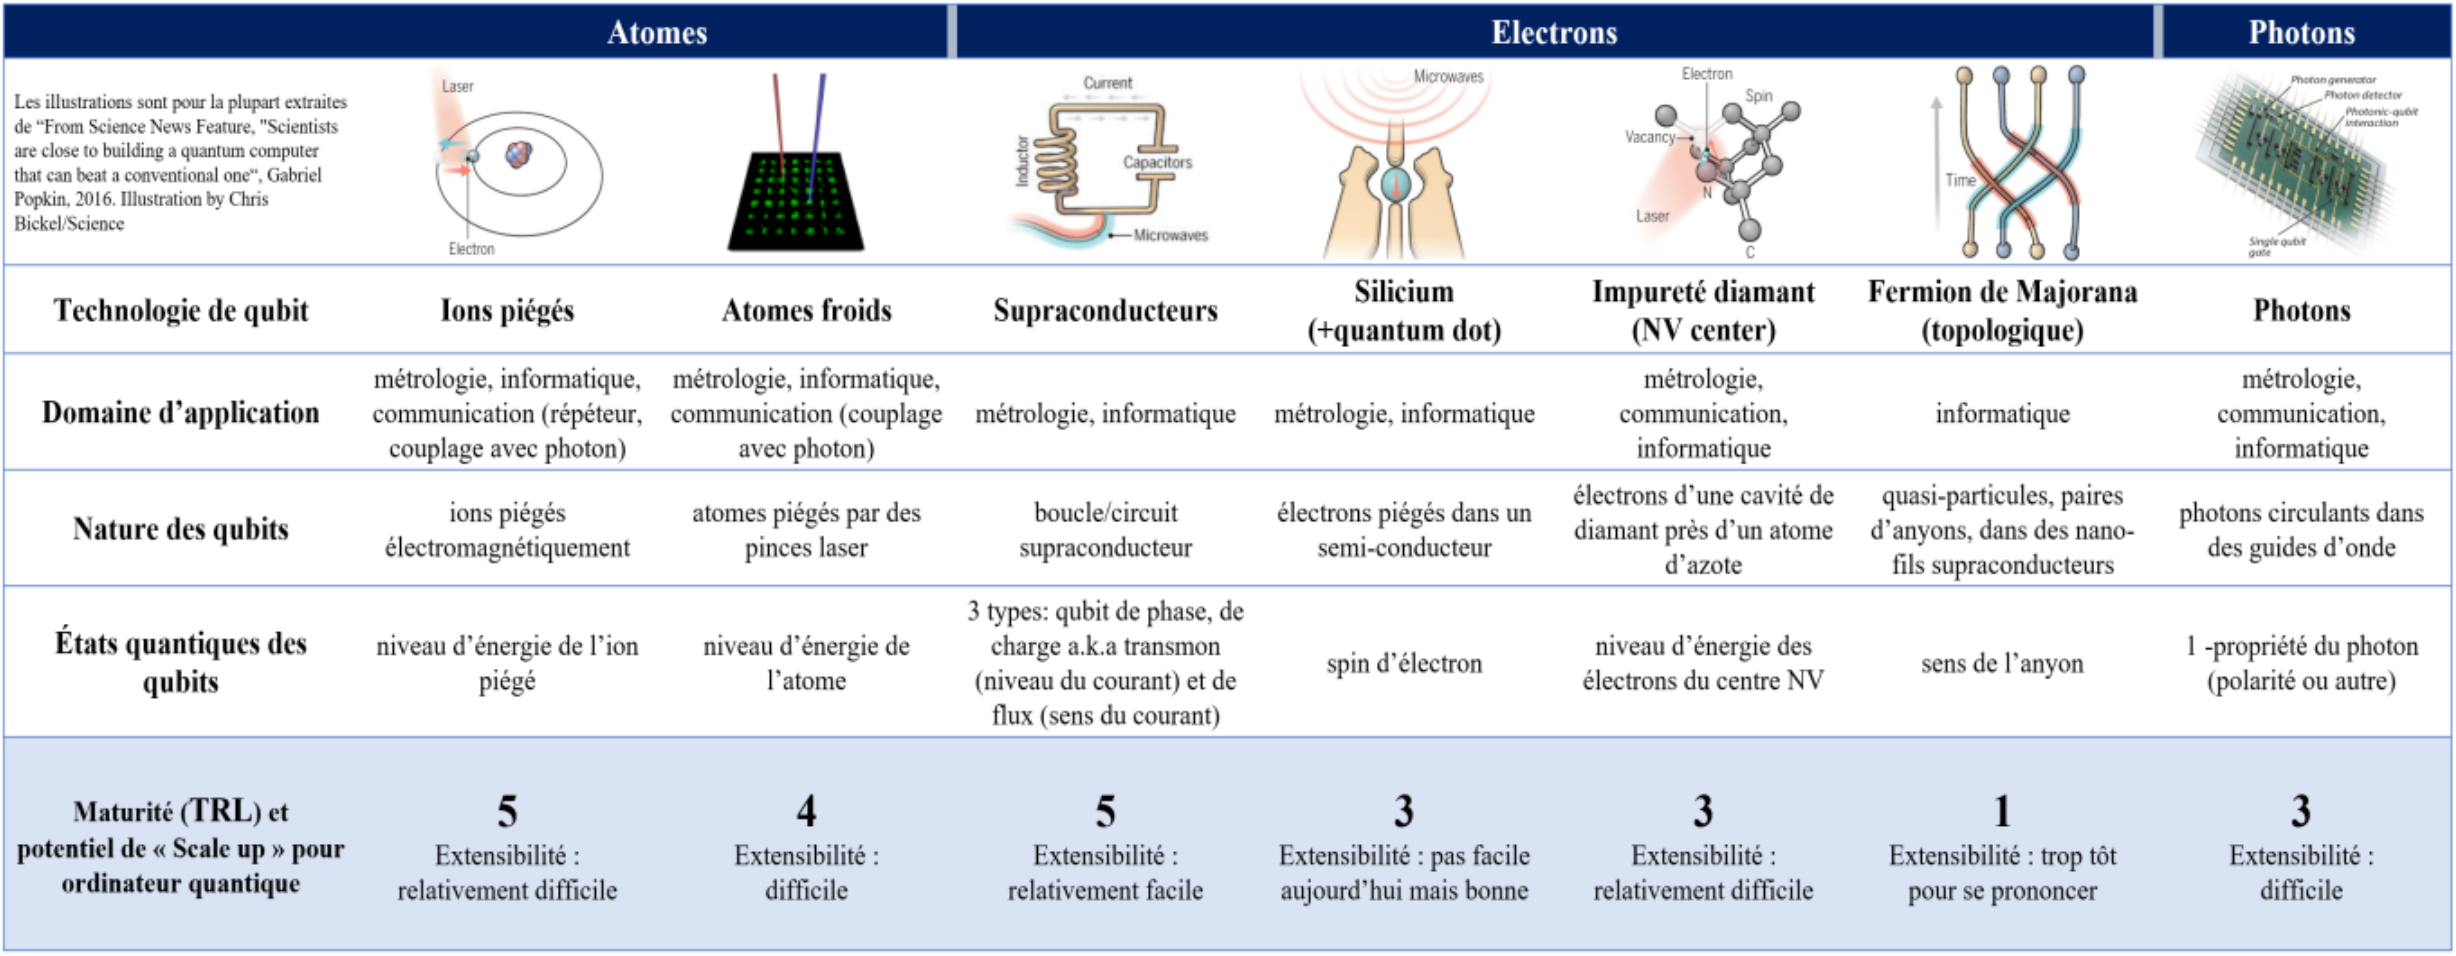
\includegraphics[width=0.7\textwidth]{qubit_how.png}
  \caption{Approcci per la realizzazione di qubit}
  \label{fig:qubit_how}
\end{figure}

Tra tutti i più utilizzati dai produttori come IBM, Google, Rigetti sono:

\begin{description}
  \item[Ioni intrappolati di un atomo] In questa tipologia di approccio, vengono costruite delle cosiddette \textit{ion trap} o trappole di ioni. Il loro scopo è trattenere all'interno degli ioni, come ad esempio un atomo di calcio che tramite l'utilizzo di un raggio laser è stato privato di uno dei due elettroni più esterni. Un chip costruito con questo approccio dei qubit è molto simile ai chip di cui sono composte le CPU classiche: si tratta infatti di un chip composto di oro su cui sono presenti gli ioni di calcio e al di sopra di essi, circa ad una distanza pari al diametro di un capelli, è presente un sottile strato di oro che alternando appositamente il suo campo magnetico, riesce a tenere gli ioni nella loro posizione ed evitare che fuoriescano (da qui si capisce il termine ion trap). \\
  Come è possibile trattare questi ioni come qubit? Innanzitutto, gli ioni naturalmente seguono i principi della meccanica quantistica, ed è possibile ottenere i due stati base di un qubit tramite l'utilizzo dello spin, presente in ogni atomo, che rappresenta una intrinseca forma di momento angolare di una particella elementare. Possiamo immaginare lo spin dell'elettrone del nostro atomo di calcio come un magnete: il nord può puntare verso l'alto, ottenendo un qubit in uno stato \(|1\rangle\) che in questo caso corrisponde a \(|\uparrow\rangle\), oppure verso il basso, ottenendo uno stato \(|0\rangle\) corrispondente a \(|\downarrow\rangle\). Per passare fra lo stato \(|\uparrow\rangle\) e \(|\downarrow\rangle\), basta utilizzare delle microonde che hanno l'effetto di ruotare lo spin dell'elettrone. È possibile quindi ruotare fermarci in un qualsiasi stato compreso fra i due spin, ottenendo quella che abbiamo in precedenza chiamato superposizione.
  \item[Superconduttori] L'approccio che utilizza i superconduttori per costruire i qubit viene utilizzato ad esempio nei computer quantistici di Google o IBM. Proprio con questo metodo di costruzione, nel 2016 Google ha annunciato di aver raggiunto la Quantum Supremacy \cite{quantum_supremacy}, cioè è stato risolto un problema che nessun calcolatore classico potrebbe risolvere in un ragionevole lasso di tempo, utilizzando un computer quantistico a 56 qubit, prodotti con questo approccio. Un superconduttore è un particolare materiale che raffreddato ad una temperatura molto vicina allo zero assoluto (0K oppure -273.15C) annulla la sua resistività elettrica completamente e grazie a queste particolari caratteristiche risulta adatto per essere utilizzato come qubit.
\end{description}